\documentclass[11pt,a4paper]{report}
\usepackage[textwidth=37em,vmargin=30mm]{geometry}
\usepackage{calc,xunicode,amsmath,amssymb,paralist,enumitem,tabu,booktabs,datetime2,xeCJK,xeCJKfntef,listings}
\usepackage{tocloft,fancyhdr,tcolorbox,xcolor,graphicx,eso-pic,xltxtra,xelatexemoji}

\newcommand{\envyear}[0]{2025}
\newcommand{\envdatestr}[0]{2025-04-01}
\newcommand{\envfinaldir}[0]{webdb/2025/20250401/final}

\usepackage[hidelinks]{hyperref}
\hypersetup{
    colorlinks=false,
    pdfpagemode=FullScreen,
    pdftitle={Web Digest - \envdatestr}
}

\setlength{\cftbeforechapskip}{10pt}
\renewcommand{\cftchapfont}{\rmfamily\bfseries\large\raggedright}
\setlength{\cftbeforesecskip}{2pt}
\renewcommand{\cftsecfont}{\sffamily\small\raggedright}

\setdefaultleftmargin{2em}{2em}{1em}{1em}{1em}{1em}

\usepackage{xeCJK,xeCJKfntef}
\xeCJKsetup{PunctStyle=plain,RubberPunctSkip=false,CJKglue=\strut\hskip 0pt plus 0.1em minus 0.05em,CJKecglue=\strut\hskip 0.22em plus 0.2em}
\XeTeXlinebreaklocale "zh"
\XeTeXlinebreakskip = 0pt


\setmainfont{Brygada 1918}
\setromanfont{Brygada 1918}
\setsansfont{IBM Plex Sans}
\setmonofont{JetBrains Mono NL}
\setCJKmainfont{Noto Serif CJK SC}
\setCJKromanfont{Noto Serif CJK SC}
\setCJKsansfont{Noto Sans CJK SC}
\setCJKmonofont{Noto Sans CJK SC}

\setlength{\parindent}{0pt}
\setlength{\parskip}{8pt}
\linespread{1.15}

\lstset{
	basicstyle=\ttfamily\footnotesize,
	numbersep=5pt,
	backgroundcolor=\color{black!5},
	showspaces=false,
	showstringspaces=false,
	showtabs=false,
	tabsize=2,
	captionpos=b,
	breaklines=true,
	breakatwhitespace=true,
	breakautoindent=true,
	linewidth=\textwidth
}






\newcommand{\coverpic}[2]{
    % argv: itemurl, authorname
    Cover photo by #2~~(\href{#1}{#1})
}
\newcommand{\makeheader}[0]{
    \begin{titlepage}
        % \newgeometry{hmargin=15mm,tmargin=21mm,bmargin=12mm}
        \begin{center}
            
            \rmfamily\scshape
            \fontspec{BaskervilleF}
            \fontspec{Old Standard}
            \fontsize{59pt}{70pt}\selectfont
            WEB\hfill DIGEST
            
            \vfill
            % \vskip 30pt
            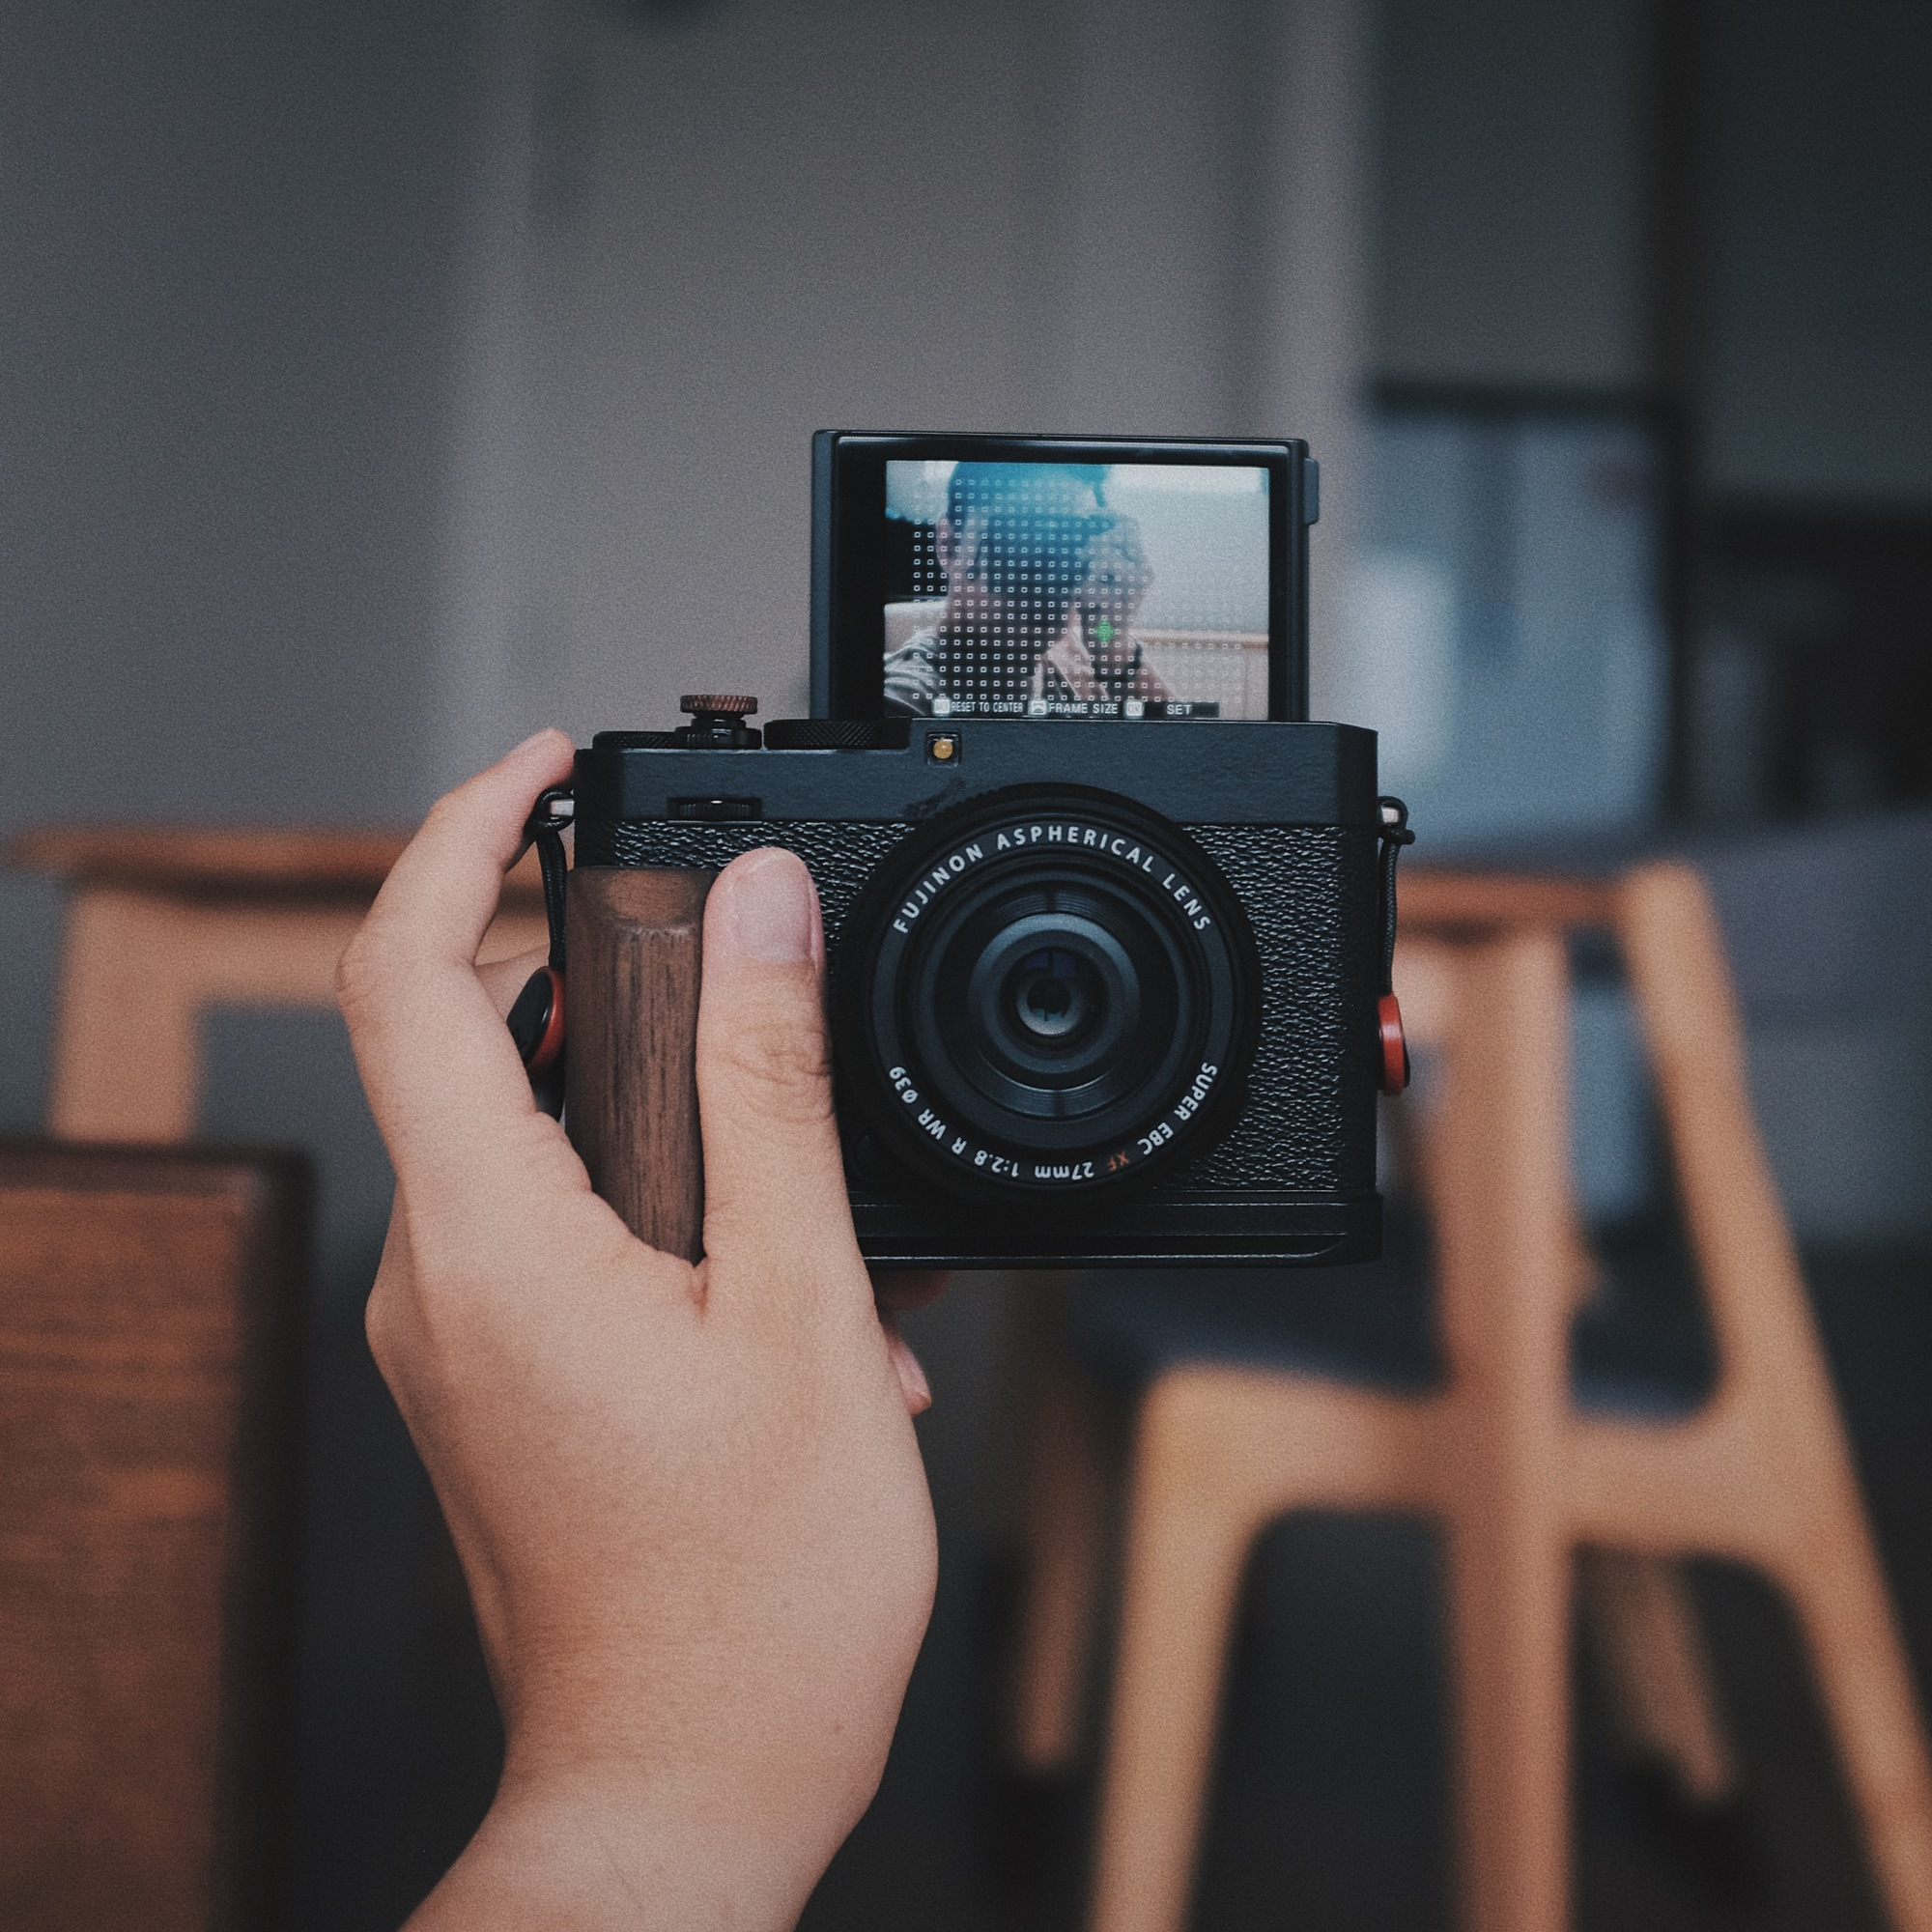
\includegraphics[width=\linewidth]{\envfinaldir/coverpic-prod.jpg}\par
            % \vskip 30pt
            \vfill

            \normalsize\rmfamily\scshape
            \copyright{} The Web Digest Project \hfill\large \envdatestr
        \end{center}
    \end{titlepage}
    % \restoregeometry
}
\newcommand{\simplehref}[1]{%
    \textcolor{blue!80!green}{\href{#1}{#1}}%
}
\renewcommand{\contentsname}{\center\Huge\sffamily\bfseries Contents\par\vskip 20pt}
\newcounter{ipartcounter}
\setcounter{ipartcounter}{0}
\newcommand{\ipart}[1]{
    % \vskip 20pt
    \clearpage
    \stepcounter{ipartcounter}
    \phantomsection
    \addcontentsline{toc}{chapter}{#1}
    % \begin{center}
    %     \Huge
    %     \sffamily\bfseries
    %     #1
    % \end{center}
    % \vskip 20pt plus 7pt
}
\newcounter{ichaptercounter}
\setcounter{ichaptercounter}{0}
\newcommand{\ichapter}[1]{
    % \vskip 20pt
    \clearpage
    \stepcounter{ichaptercounter}
    \phantomsection
    \addcontentsline{toc}{section}{\numberline{\arabic{ichaptercounter}}#1}
    \begin{center}
        \Huge
        \sffamily\bfseries
        #1
    \end{center}
    \vskip 20pt plus 7pt
}
\newcommand{\entrytitlefont}[1]{\subsection*{\raggedright\Large\sffamily\bfseries#1}}
\newcommand{\entryitemGeneric}[2]{
    % argv: title, url
    \parbox{\linewidth}{
        \entrytitlefont{#1}\par\vskip 5pt
        \footnotesize\ttfamily\mdseries
        \simplehref{#2}
    }\vskip 11pt plus 11pt minus 1pt
}
\newcommand{\entryitemGithub}[3]{
    % argv: title, url, desc
    \parbox{\linewidth}{
        \entrytitlefont{#1}\par\vskip 5pt
        \footnotesize\ttfamily\mdseries
        \simplehref{#2}\par\vskip 5pt
        \small\rmfamily\mdseries#3
    }\vskip 11pt plus 11pt minus 1pt
}
\newcommand{\entryitemAp}[3]{
    % argv: title, url, desc
    \parbox{\linewidth}{
        \entrytitlefont{#1}\par\vskip 5pt
        \footnotesize\ttfamily\mdseries
        \simplehref{#2}\par\vskip 5pt
        \small\rmfamily\mdseries#3
    }\vskip 11pt plus 11pt minus 1pt
}
\newcommand{\entryitemHackernews}[3]{
    % argv: title, hnurl, rawurl
    % \parbox{\linewidth}{
    %     \entrytitlefont{#1}\par\vskip 5pt
    %     \footnotesize\ttfamily\mdseries
    %     \simplehref{#3}\par
    %     \textcolor{black!50}{\href{#2}{#2}}
    % }\vskip 11pt plus 11pt minus 1pt
    \begin{minipage}{\linewidth}
            \entrytitlefont{#1}\par\vskip 5pt
            \footnotesize\ttfamily\mdseries
            \simplehref{#3}\par
            \textcolor{black!50}{\href{#2}{#2}}
    \end{minipage}\par\vskip 11pt plus 11pt minus 1pt
}







\begin{document}

\makeheader

\tableofcontents\clearpage




\ipart{Developers}
\ichapter{Hacker News}
\entryitemTwoLinks{JEP Draft: Prepare to Make Final Mean Final}{https://news.ycombinator.com/item?id=43538919}{https://openjdk.org/jeps/8349536}

\entryitemTwoLinks{Kagi for Kids}{https://news.ycombinator.com/item?id=43538338}{https://help.kagi.com/kagi/plans/family-plan.html\#kidslogin}

\entryitemTwoLinks{Honey has now lost 4M Chrome users after shady tactics were revealed}{https://news.ycombinator.com/item?id=43538113}{https://9to5google.com/2025/03/31/honey-extension-users-dropped-chrome-march-2025/}

\entryitemTwoLinks{France fines Apple €150M for ``excessive'' pop-ups that let users reject tracking}{https://news.ycombinator.com/item?id=43537593}{https://arstechnica.com/tech-policy/2025/03/france-fines-apple-e150m-for-excessive-pop-ups-that-let-users-reject-tracking/}

\entryitemTwoLinks{MLB says Yankees' new "torpedo bats" are legal and likely coming}{https://news.ycombinator.com/item?id=43536146}{https://thelibertyline.com/2025/03/30/yankees-new-torpedo-bat/}

\entryitemTwoLinks{Oracle attempt to hide cybersecurity incident from customers?}{https://news.ycombinator.com/item?id=43535953}{https://doublepulsar.com/oracle-attempt-to-hide-serious-cybersecurity-incident-from-customers-in-oracle-saas-service-9231c8daff4a}

\entryitemTwoLinks{Turso SQLite Offline Sync Public Beta}{https://news.ycombinator.com/item?id=43535943}{https://turso.tech/blog/turso-offline-sync-public-beta}

\entryitemTwoLinks{Browsercraft: Java Minecraft in the browser}{https://news.ycombinator.com/item?id=43535769}{https://browsercraft.cheerpj.com/}

\entryitemTwoLinks{It's not mold, it's calcium lactate (2018)}{https://news.ycombinator.com/item?id=43535688}{https://www.thephcheese.com/theres-white-stuff-growing-on-your-cheese-that-isnt-mold}

\entryitemTwoLinks{AI agents: Less capability, more reliability, please}{https://news.ycombinator.com/item?id=43535653}{https://www.sergey.fyi/articles/reliability-vs-capability}

\entryitemTwoLinks{Marine Le Pen banned from running in 2027 and given four-year sentence}{https://news.ycombinator.com/item?id=43534140}{https://www.theguardian.com/world/live/2025/mar/31/france-marine-le-pen-embezzlement-verdict-europe-news-live}

\entryitemTwoLinks{Gemini 2.5 Pro vs. Claude 3.7 Sonnet: Coding Comparison}{https://news.ycombinator.com/item?id=43534029}{https://composio.dev/blog/gemini-2-5-pro-vs-claude-3-7-sonnet-coding-comparison/}

\entryitemTwoLinks{The Egg (By Andy Weir)}{https://news.ycombinator.com/item?id=43533826}{https://www.galactanet.com/oneoff/theegg.html}

\entryitemTwoLinks{Compiler Options Hardening Guide for C and C++}{https://news.ycombinator.com/item?id=43533516}{https://best.openssf.org/Compiler-Hardening-Guides/Compiler-Options-Hardening-Guide-for-C-and-C++.html}

\entryitemTwoLinks{Things I Won't Work With: Dioxygen Difluoride (2010)}{https://news.ycombinator.com/item?id=43533496}{https://www.science.org/content/blog-post/things-i-won-t-work-dioxygen-difluoride}

\entryitemTwoLinks{The demoscene as a UNESCO heritage in Sweden}{https://news.ycombinator.com/item?id=43533362}{https://www.goto80.com/the-demoscene-as-a-unesco-heritage-in-sweden}

\entryitemTwoLinks{James Webb Space Telescope reveals that most galaxies rotate clockwise}{https://news.ycombinator.com/item?id=43533306}{https://www.smithsonianmag.com/smart-news/james-webb-space-telescope-reveals-that-most-galaxies-rotate-clockwise-180986224/}

\entryitemTwoLinks{ToS;DR}{https://news.ycombinator.com/item?id=43533096}{https://tosdr.org/en}

\entryitemTwoLinks{Show HN: WhatsApp MCP Server}{https://news.ycombinator.com/item?id=43532967}{https://github.com/lharries/whatsapp-mcp}

\entryitemTwoLinks{The <select> element can now be customized with CSS}{https://news.ycombinator.com/item?id=43532830}{https://developer.chrome.com/blog/a-customizable-select}\ichapter{Phoronix}
\entryitemGeneric{\hskip 0pt{}Wayland Is On Track For A Very Exciting 2025}{https://www.phoronix.com/news/Wayland-Q1-2025}

\entryitemGeneric{\hskip 0pt{}Linux 6.15 Perf Tooling Introduces New Support For Latency Profiling}{https://www.phoronix.com/news/Linux-6.15-Perf-Tools-Latency}

\entryitemGeneric{\hskip 0pt{}wlroots Merges Wayland Color Management / HDR Support}{https://www.phoronix.com/news/wlroots-color-management}

\entryitemGeneric{\hskip 0pt{}Dasharo Platform Driver Aims To Enhance The Experience Using This Coreboot Downstream}{https://www.phoronix.com/news/Dasharo-ACPI-Platform-Driver}

\entryitemGeneric{\hskip 0pt{}Redis-Forked Valkey 8.1 Released - Turns To AVX2 For Better Performance}{https://www.phoronix.com/news/Valkey-8.1-Released}

\entryitemGeneric{\hskip 0pt{}Linux 6.15 exFAT Can Delete Files Much Faster: 4+ Minutes To 1.6 Second Optimization}{https://www.phoronix.com/news/Linux-6.15-exFAT}

\entryitemGeneric{\hskip 0pt{}AMD Software Advancements, RDNA4 \& Ryzen 9900X3D Series Excited Linux Users In Q1}{https://www.phoronix.com/news/AMD-Q1-2025-Highlights}

\entryitemGeneric{\hskip 0pt{}FreeBSD On Laptops Sees New Power Management Driver, WiFi 4 / WiFi 5 Progress}{https://www.phoronix.com/news/FreeBSD-Laptops-Feb-2025}

\entryitemGeneric{\hskip 0pt{}Firefox 137 Release Brings VA-API Accelerated H.265 On Linux}{https://www.phoronix.com/news/Firefox-137-Available}\ichapter{Dribbble}
\entryitemGeneric{\hskip 0pt{}FG}{https://dribbble.com/shots/25842733-FG}

\entryitemGeneric{\hskip 0pt{}Let down your hair}{https://dribbble.com/shots/25844844-Let-down-your-hair}

\entryitemGeneric{\hskip 0pt{}Chat GPT 4 Branding Concept}{https://dribbble.com/shots/25844194-Chat-GPT-4-Branding-Concept}

\entryitemGeneric{\hskip 0pt{}I'm leaving Dribbble. After 15 years.}{https://dribbble.com/shots/25836899-I-m-leaving-Dribbble-After-15-years}

\entryitemGeneric{\hskip 0pt{}Weylix Logo Design - W Letter Monogram, Wave}{https://dribbble.com/shots/25834720-Weylix-Logo-Design-W-Letter-Monogram-Wave}

\entryitemGeneric{\hskip 0pt{}BB}{https://dribbble.com/shots/25834486-BB}

\entryitemGeneric{\hskip 0pt{}Banking Mobile App Design}{https://dribbble.com/shots/25829959-Banking-Mobile-App-Design}

\entryitemGeneric{\hskip 0pt{}The Rocky token landing page}{https://dribbble.com/shots/25827682-The-Rocky-token-landing-page}

\entryitemGeneric{\hskip 0pt{}Suffo - Real Estate Landing page Animation}{https://dribbble.com/shots/25829238-Suffo-Real-Estate-Landing-page-Animation}

\entryitemGeneric{\hskip 0pt{}Mishto Logo Design}{https://dribbble.com/shots/25830165-Mishto-Logo-Design}

\entryitemGeneric{\hskip 0pt{}Big gestures}{https://dribbble.com/shots/25826632-Big-gestures}

\entryitemGeneric{\hskip 0pt{}Proven UI/UX design, User Interface experience}{https://dribbble.com/shots/25819444-Proven-UI-UX-design-User-Interface-experience}

\entryitemGeneric{\hskip 0pt{}Dog + Play Button}{https://dribbble.com/shots/25809362-Dog-Play-Button}

\entryitemGeneric{\hskip 0pt{}Pricefy Logo Design - Mountains, Chart, Graph, Sun}{https://dribbble.com/shots/25824720-Pricefy-Logo-Design-Mountains-Chart-Graph-Sun}

\entryitemGeneric{\hskip 0pt{}Yada Yada Yada}{https://dribbble.com/shots/25826541-Yada-Yada-Yada}

\entryitemGeneric{\hskip 0pt{}Music Road}{https://dribbble.com/shots/25827168-Music-Road}

\entryitemGeneric{\hskip 0pt{}Illustration}{https://dribbble.com/shots/25822720-Illustration}

\entryitemGeneric{\hskip 0pt{}Crypto Portfolio Tracker App}{https://dribbble.com/shots/25820014-Crypto-Portfolio-Tracker-App}

\entryitemGeneric{\hskip 0pt{}Gemini Rebrand}{https://dribbble.com/shots/25821410-Gemini-Rebrand}

\entryitemGeneric{\hskip 0pt{}Cyber Extrusion (Merch/Custom T-shirt)}{https://dribbble.com/shots/25821987-Cyber-Extrusion-Merch-Custom-T-shirt}

\entryitemGeneric{\hskip 0pt{}FCKD - Part 2}{https://dribbble.com/shots/25817864-FCKD-Part-2}

\entryitemGeneric{\hskip 0pt{}ROOT BEER}{https://dribbble.com/shots/25815759-ROOT-BEER}

\entryitemGeneric{\hskip 0pt{}Summer time}{https://dribbble.com/shots/25821066-Summer-time}

\entryitemGeneric{\hskip 0pt{}SafeHold ledeger responsive}{https://dribbble.com/shots/25817185-SafeHold-ledeger-responsive}


\ipart{Developers~~~~(zh-Hans)}
\ichapter{Solidot}
\entryitemGeneric{\hskip 0pt{}鱼也会使用工具}{https://www.solidot.org/story?sid=80927}

\entryitemGeneric{\hskip 0pt{}接受调查的美国研究人员四分之三考虑离开}{https://www.solidot.org/story?sid=80926}

\entryitemGeneric{\hskip 0pt{}北极海冰范围冬季峰值 47 年来最低}{https://www.solidot.org/story?sid=80925}

\entryitemGeneric{\hskip 0pt{}计算机科学家 Xiaofeng Wang 失踪,其家被 FBI 搜查}{https://www.solidot.org/story?sid=80923}

\entryitemGeneric{\hskip 0pt{}Akamai 宣布托管 kernel.org 核心基础设施}{https://www.solidot.org/story?sid=80922}

\entryitemGeneric{\hskip 0pt{}火星尘埃可能会对宇航员构成健康威胁}{https://www.solidot.org/story?sid=80921}

\entryitemGeneric{\hskip 0pt{}法航因乘客手机丢失而被迫返航}{https://www.solidot.org/story?sid=80920}

\entryitemGeneric{\hskip 0pt{}科学家可能找到了阻止秃顶的方法}{https://www.solidot.org/story?sid=80919}

\entryitemGeneric{\hskip 0pt{}天文学家首度确认海王星存在极光现象}{https://www.solidot.org/story?sid=80918}

\entryitemGeneric{\hskip 0pt{}未来的 Windows 版本将必须要有网络连接和 Microsoft Account 账号才能安装}{https://www.solidot.org/story?sid=80917}

\entryitemGeneric{\hskip 0pt{}涉及 Waymos 的绝大多数车祸都是人类司机引起的}{https://www.solidot.org/story?sid=80916}\ichapter{V2EX}
\entryitemGeneric{\hskip 0pt{}[问与答] 移动的 200 多 g 大流量卡什么时候会有?}{https://www.v2ex.com/t/1122441}

\entryitemGeneric{\hskip 0pt{}[Apple] Mac mini 内存选配求助}{https://www.v2ex.com/t/1122440}

\entryitemGeneric{\hskip 0pt{}[程序员] [分享] 从 Android 开发到全栈: 48 小时左右用 AI 打造吉卜力风格绘图网站}{https://www.v2ex.com/t/1122439}

\entryitemGeneric{\hskip 0pt{}[NAS] 寻找一款支持 SSD 的 NAS 升级现有 DS218+}{https://www.v2ex.com/t/1122438}

\entryitemGeneric{\hskip 0pt{}[分享发现] Folo (Follow) 安卓 Android App 预计一个月内上线}{https://www.v2ex.com/t/1122437}

\entryitemGeneric{\hskip 0pt{}[Apple] iOS/iPadOS 上的浏览器下载个普通的视频好麻烦}{https://www.v2ex.com/t/1122436}

\entryitemGeneric{\hskip 0pt{}[问与答] 室内客厅墙上有一个免费不间断的 12V1A 的电源,可以怎么利用一下}{https://www.v2ex.com/t/1122435}

\entryitemGeneric{\hskip 0pt{}[问与答] 如何优雅的更新 1panel 上的 go 服务端网站}{https://www.v2ex.com/t/1122434}

\entryitemGeneric{\hskip 0pt{}[汽车] GLC 300 和 YU7 怎么选?}{https://www.v2ex.com/t/1122433}

\entryitemGeneric{\hskip 0pt{}[MacBook Air] Macbook Air 熄屏休眠时间久了之后 Touch ID 解锁闪屏}{https://www.v2ex.com/t/1122432}

\entryitemGeneric{\hskip 0pt{}[分享创造] 小红书 | 图文,视频,评论 浏览与导出工具}{https://www.v2ex.com/t/1122430}

\entryitemGeneric{\hskip 0pt{}[问与答] 使用 handbrake 大菠萝转码 CPU 都是满载, 如何降低 CPU 占用?}{https://www.v2ex.com/t/1122429}

\entryitemGeneric{\hskip 0pt{}[游戏] MacBook Pro M4 上可以玩原神 b 服吗?}{https://www.v2ex.com/t/1122427}

\entryitemGeneric{\hskip 0pt{}[Android] 为啥 rednote 支持 fcm,而小红书就不支持了呢?}{https://www.v2ex.com/t/1122426}

\entryitemGeneric{\hskip 0pt{}[分享发现] 发现一个可以免费生成 AI 图片 / 视频的网站}{https://www.v2ex.com/t/1122425}

\entryitemGeneric{\hskip 0pt{}[程序员] 崩溃了, Mac 外接俩显示器, USBC+HDMI, USBC 唤醒三天两头不好使,只能重启}{https://www.v2ex.com/t/1122424}

\entryitemGeneric{\hskip 0pt{}[分享创造] v2ex mcp server}{https://www.v2ex.com/t/1122422}

\entryitemGeneric{\hskip 0pt{}[OpenWrt] 分享我的 SS 速度测试脚本以及结果(WR30U ImmortalWrt)}{https://www.v2ex.com/t/1122421}

\entryitemGeneric{\hskip 0pt{}[Windows] 请问搜索服务下 windows 输入体验进程是干什么的?}{https://www.v2ex.com/t/1122420}

\entryitemGeneric{\hskip 0pt{}[分享创造] 做了个 brat 专辑风格封面生成工具}{https://www.v2ex.com/t/1122419}

\entryitemGeneric{\hskip 0pt{}[问与答] giffgaff esim 转移到新手机 esim 失败求助}{https://www.v2ex.com/t/1122417}

\entryitemGeneric{\hskip 0pt{}[Apple] arc browser 公司新出的 dia browser 邀请 5 个人}{https://www.v2ex.com/t/1122415}

\entryitemGeneric{\hskip 0pt{}[推广] 犹豫再三,还是决定向 V 友推荐下这套《AI 编程体系课》}{https://www.v2ex.com/t/1122413}

\entryitemGeneric{\hskip 0pt{}[WordPress] ai 这么猛了,有 wp 插件生成静态 next.js 前端的吗?}{https://www.v2ex.com/t/1122412}

\entryitemGeneric{\hskip 0pt{}[生活] TBHQ 到底有毒吗?}{https://www.v2ex.com/t/1122410}

\entryitemGeneric{\hskip 0pt{}[程序员] 用 gpt4o 生成头像表情包,真是绝了。}{https://www.v2ex.com/t/1122409}

\entryitemGeneric{\hskip 0pt{}[游戏开发] 有没有懂游戏匹配实现的(以炉石传说为例),求指个路}{https://www.v2ex.com/t/1122408}

\entryitemGeneric{\hskip 0pt{}[问与答] Macbook Air M4 适不适合搞大前端开发}{https://www.v2ex.com/t/1122407}

\entryitemGeneric{\hskip 0pt{}[问与答] 话说有 macos 极客吗上个帖子被移到水区了,以下是新补充}{https://www.v2ex.com/t/1122406}

\entryitemGeneric{\hskip 0pt{}[互联网] 现在用``什么值得买''的人还多吗?为什么不可以做一个替代他?他有什么壁垒?}{https://www.v2ex.com/t/1122405}

\entryitemGeneric{\hskip 0pt{}[程序员] 如何利用 API 对接 AI(比如 deepseek),实现读取数据库里面的内容,根据用户的提问,返回推荐的文章}{https://www.v2ex.com/t/1122404}

\entryitemGeneric{\hskip 0pt{}[Chrome] 我用 brunch 刷了 chromeos 登录时提示是企业,要授权怎么办?}{https://www.v2ex.com/t/1122403}

\entryitemGeneric{\hskip 0pt{}[分享创造] 基于 cloudflare worker ai 在 IF 中开发了一个文档转换工具,可以用来给知识库提供语料}{https://www.v2ex.com/t/1122402}

\entryitemGeneric{\hskip 0pt{}[CentOS] vscode 的 remote-ssh 还支持 centos7 吗?}{https://www.v2ex.com/t/1122401}

\entryitemGeneric{\hskip 0pt{}[微信] 才发现微信读书阅读一天不能领取奖励了啊}{https://www.v2ex.com/t/1122400}

\entryitemGeneric{\hskip 0pt{}[程序员] TS 语言 Interface 与 Type 设计:宽松兼容与模糊规则下的程序员滥用危机}{https://www.v2ex.com/t/1122399}

\entryitemGeneric{\hskip 0pt{}[程序员] 各位大佬们,有没有好用的 jar 包加固的工具推荐}{https://www.v2ex.com/t/1122398}

\entryitemGeneric{\hskip 0pt{}[职场话题] 每天多少个小时的工作时间不会让人下班后感觉疲惫?}{https://www.v2ex.com/t/1122397}

\entryitemGeneric{\hskip 0pt{}[全球工单系统] 今日份腾讯云短信炸了}{https://www.v2ex.com/t/1122396}

\entryitemGeneric{\hskip 0pt{}[问与答] RSS 制作,对于没开 rss 的网站,有啥比较成熟稳定的生成方案?别是自己学 Python 自己造吧?}{https://www.v2ex.com/t/1122395}

\entryitemGeneric{\hskip 0pt{}[程序员] 为什么 Google 不弄个 Angular Native 这样 Angular 写 Native 界面的框架? Angular 这套设计明显更适合大型项目,企业级,架构更清晰,感觉会比 Flutter 好用得多}{https://www.v2ex.com/t/1122394}

\entryitemGeneric{\hskip 0pt{}[VXNA] 申请收录个人博客: Albert's Blog}{https://www.v2ex.com/t/1122393}

\entryitemGeneric{\hskip 0pt{}[Node.js] 同样是运行 npm run build 打包程序 cursor 比 hbx 慢 1000 倍}{https://www.v2ex.com/t/1122390}

\entryitemGeneric{\hskip 0pt{}[职场话题] 初级程序员的未来是什么}{https://www.v2ex.com/t/1122389}

\entryitemGeneric{\hskip 0pt{}[酷工作] [杭州] 淘天集团 2026 届实习生招聘}{https://www.v2ex.com/t/1122388}

\entryitemGeneric{\hskip 0pt{}[分享发现] 极简 Mac 剪贴板 App —— AegisClip}{https://www.v2ex.com/t/1122387}

\entryitemGeneric{\hskip 0pt{}[汽车] 领克 900 的车重为什么这么夸张?}{https://www.v2ex.com/t/1122386}

\entryitemGeneric{\hskip 0pt{}[OpenAI] 如何使用 Grok2 Api?}{https://www.v2ex.com/t/1122384}

\entryitemGeneric{\hskip 0pt{}[生活] 家长催婚,催相亲很有意思的一些逻辑悖论}{https://www.v2ex.com/t/1122382}

\entryitemGeneric{\hskip 0pt{}[问与答] 微信今天发布桌面端 4.0 版本了,而且还正式上线产品官网,总算是实现多桌面端统一}{https://www.v2ex.com/t/1122380}


\ipart{Generic News}







\clearpage
\leavevmode\vfill
\footnotesize

Copyright \copyright{} 2023-2025 Neruthes and other contributors.

This document is published with CC BY-NC-ND 4.0 license.

The entries listed in this newsletter may be copyrighted by their respective creators.

This newsletter is generated by the Web Digest project.

The newsletters are also delivered via Telegram channel \CJKunderline{\href{https://t.me/webdigestchannel}{https://t.me/webdigestchannel}}.\\
RSS feed is available at \CJKunderline{\href{https://webdigest.pages.dev/rss.xml}{https://webdigest.pages.dev/rss.xml}}.

This newsletter is available in PDF at
\CJKunderline{\href{https://webdigest.pages.dev/}{https://webdigest.pages.dev/}}.

The source code being used to generate this newsletter is available at\\
\CJKunderline{\href{https://github.com/neruthes/webdigest}{https://github.com/neruthes/webdigest}}.

This newsletter is also available in
\CJKunderline{\href{http://webdigest.pages.dev/readhtml/\envyear/WebDigest-20250401.html}{HTML}} and
\CJKunderline{\href{https://github.com/neruthes/webdigest/blob/master/markdown/\envyear/WebDigest-20250401.md}{Markdown}}.


\coverpic{https://unsplash.com/photos/a-palm-tree-on-a-beach-with-the-ocean-in-the-background-v3LDDBTgkkU}{Karl Moore}


\end{document}
